\chapter{Robot Design and Control Implementation}
\label{sec:ExperimentalValidation}

{
\begin{flushright}
\textit{"What I cannot create, I do not understand."} \\ 
\emph{-- Richard Phillips Feynman}
\end{flushright}
}
\vspace{10pt}

%\begin{flushright}
%\small"The test of all knowledge is experiment. Experiment is the sole judge of scientific truth." \\ \emph{Richard Phillips Feynman}
%\end{flushright}


This chapter present a novel robot prototype using DSDM actuators. The mechanical design of the DSDM actuators and robotic arm prototype and controllers implementation are described.

\begin{figure}[htp]
	\centering
		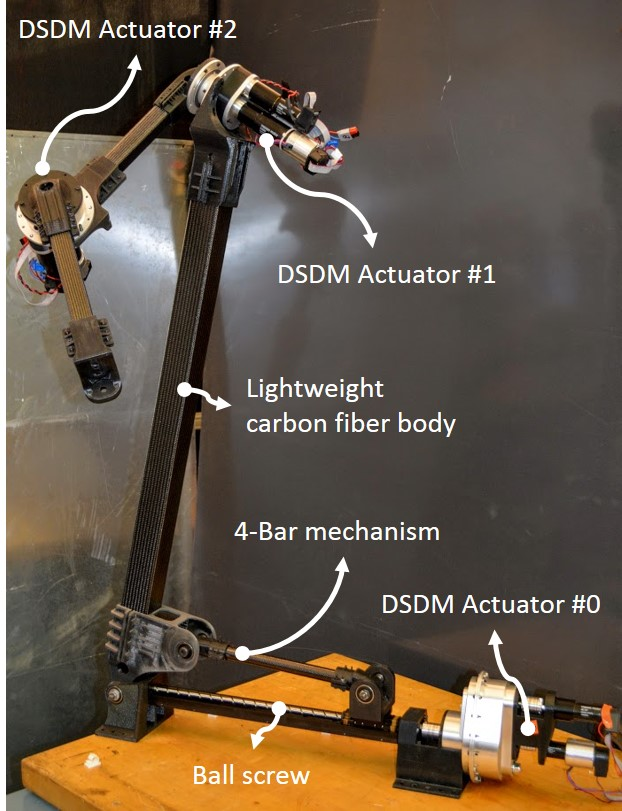
\includegraphics[width=0.90\textwidth]{arm_proto_3.jpg}
	\caption{3-DoF custom arm using 3 DSDM actuators}
	\label{fig:dsdm_arm}
\end{figure}


\section{Lightweight Arm Design}
\label{sec:DSDMArm}

A custom robotic arm using 3 DSDM actuators was designed and built, see Fig. \ref{fig:dsdm_arm}. This arm is very strong and fast for its weight when compared to traditional robotic arms. 

\section{DSDM Actuator Design}
\label{sec:ActuatorDesign}
 
Three actuator prototypes were developed, with different mechanical advantage for the shoulder, elbow and wrist DoF of the arm. All of them use discrete components for the ease of implementation and modularity. The shoulder actuator is designed to drive a ballscrew, for a large efficient reduction, and the others actuators are embedded into revolute joints. 

\subsubsection{Revolute Joint Actuators}

Fig. \ref{fig:dsdm_act} shows the prototype for a revolute DSDM actuator. The elbow and wrist actuator have the same design with the exception of using different gearing ratios.

\begin{figure}[htp]
	\centering
		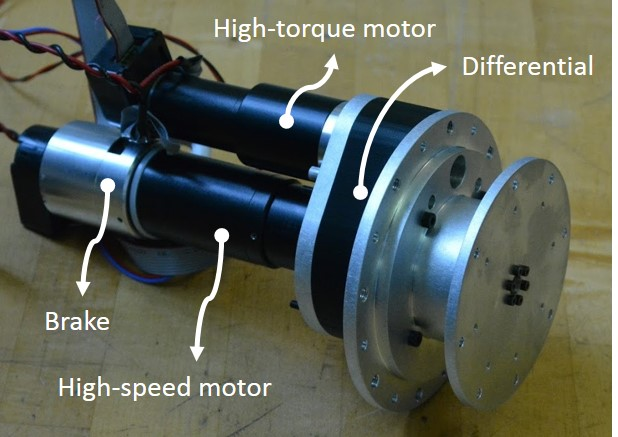
\includegraphics[width=0.75\textwidth]{dsdm_proto_2.jpg}
	\caption{Revolute joint DSDM actuator prototype } %Max continuous torque of 40 Nm and maximum velocity of 100 RPM
	\label{fig:dsdm_act}
\end{figure}

The prototype consist of a custom housing holding both the differential and support bearing for the output. Discrete \textit{Maxon} motors with gear-head of the serie GP32 can be attached to the back of the gear-box. It is thus possible to attach a wide-range of motor, from 20 watts to 200 watts, and with a wide range of additional gear-head reduction. 

\begin{figure}[htbp]
	\centering
		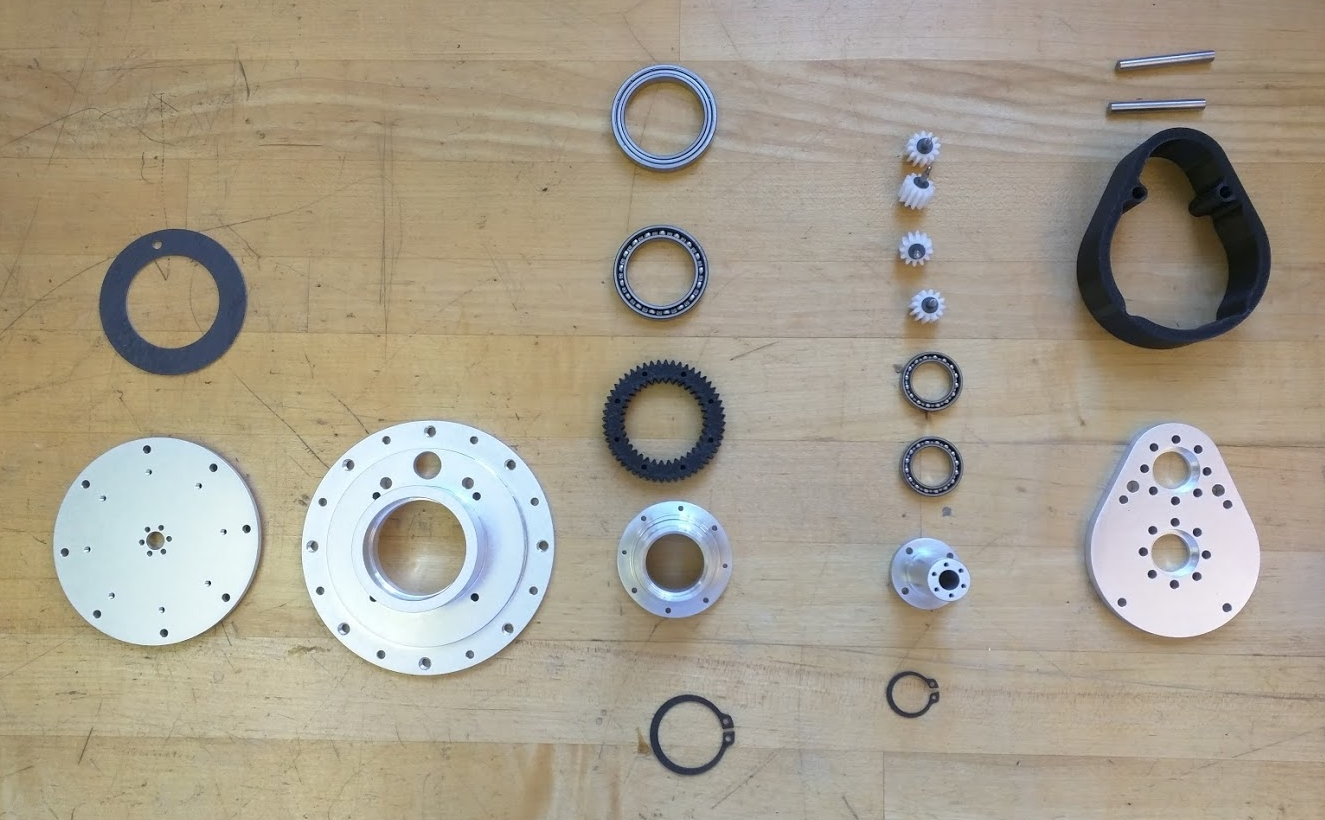
\includegraphics[width=0.90\textwidth]{dsdm_parts.jpg}
	\caption{Dsdm parts}
	\label{fig:dsdm_parts}
\end{figure}


The differential in the gear-box is implemented using a planetary gear-train, where is ring-gear is mounted on bearings. The planet-carrier unit is connected to the actuator output, the sun-gear is connected to the high-speed motor, and the ring-gear is driven by an additional reduction stage connected to the high-force motor. Fig. \ref{fig:dsdm_section} show the internal architecture of the system.


\begin{figure}[htp]
	\centering
		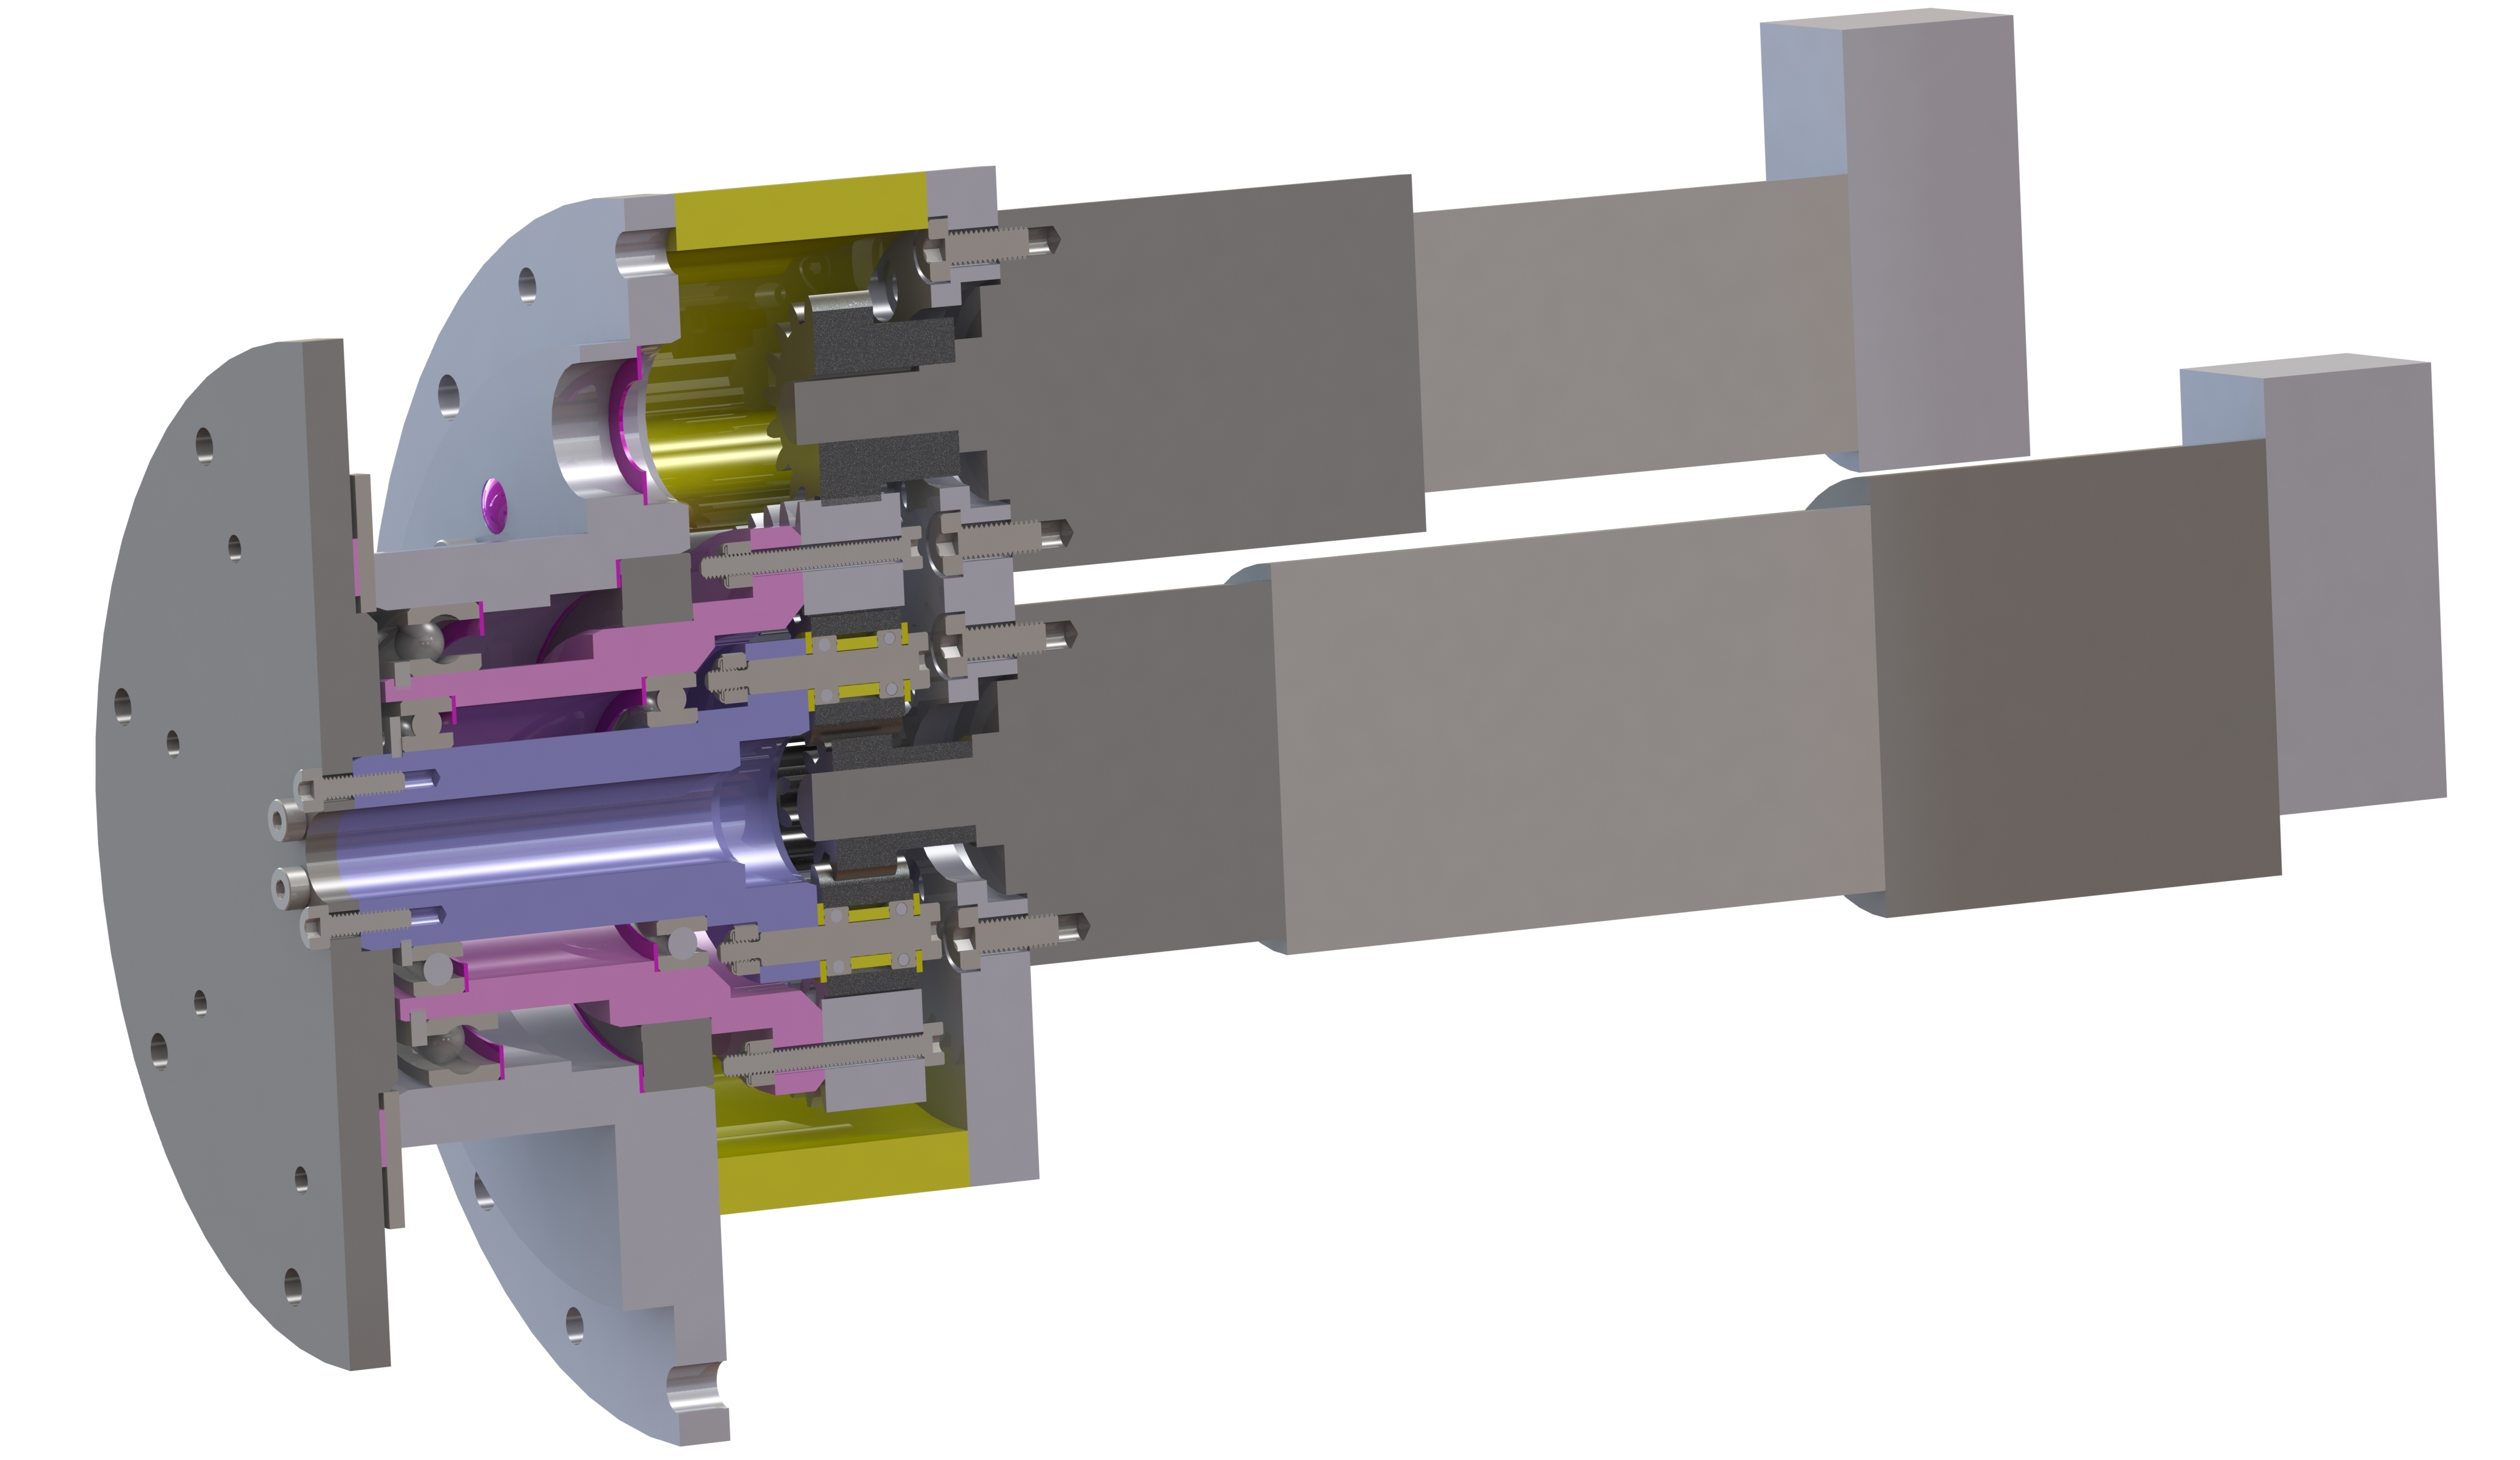
\includegraphics[width=0.95\textwidth]{metal_DSDM_section_view.jpg}
	\caption{Section view of the CAD model of the actuator prototype} %Max continuous torque of 40 Nm and maximum velocity of 100 RPM
	\label{fig:dsdm_section}
\end{figure}


\subsubsection{Linear Actuator}

To achieve the large reduction needed for the shoulder actuator of the robot, while keeping the mechanism back-drivable during high-speed mode, a large-lead ballscrew linear stage is used. 


\subsubsection{Specifications}



%Shown in Fig. \ref{fig:arm_proto}, a 3-DoF robotic arm using variable gear-ratio actuators has been designed and custom built. The variable gear-ratio actuators consist of dual-speed dual-motor (DSDM) actuators, as shown in Fig. \ref{fig:dsdm_cad}. Those actuators have two discrete operating modes, one for high-speed operation, and the other for low-speed, high-load operation, where the net gear-ratios are more than 20-times different. DSDM actuators are lighter than would be single motors sized to reach the same maximum speed and maximum torque \cite{girard_two-speed_2015}. Also, the dual-motor architecture has the advantages of allowing fast and seamless gear-shifts, by doing the synchronization in the nullspace, which support the modeling assumption discussed at sec. \ref{sec:mod}. 


%For instance, the actuation and joint unit shown at Fig. \ref{fig:dsdm_cad} weights 1.5 Kg (un-optimized first prototype), can reach a 100 RPM velocity and a maximum continuous torque of 40 Nm (based on the very conservative torque rating of Maxon motor [ref] )

%\begin{figure}[htp]
	%\centering
		%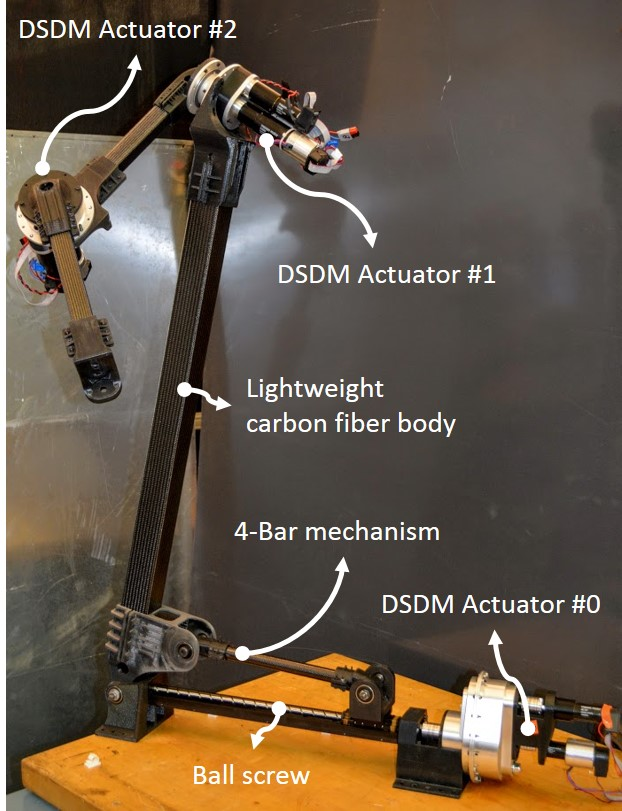
\includegraphics[width=0.45\textwidth]{arm_proto_3.jpg}
	%\caption{Prototype 3-DOF arm with variable gear-ratio actuators}
	%\label{fig:arm_proto}
%\end{figure}



\section{Control Implementation}
\label{sec:ControlSoftwareArchitecture}

The control algorithms are implemented on a computer using ROS \cite{quigley_ros:_2009}, the trajectory generation algorithm and the R* Computed Torque controller are written in \textit{Python}. The computer is communicating over USB with open-source \textit{Flexsea} motor-drivers \cite{duval_flexsea-execute:_2016} that handle the low-level current loops. The trajectory is generated offline in advance and loaded in memory upon initialization. The main R* control loop is running at a 500 Hz sampling rate. The low-level actuator controllers, receiving the torque and gear-ratio set-points, communicating with both motor drivers and handling the gear-shifting process (see Fig. \ref{fig:control_achitecture}), are ... TODO

%also implemented in \textit{Python} and use the algorithm described in \cite{girard_two-speed_2015}. Transition from one gear-ratio to another are found to be consistently under 50 ms.

\subsection{Controller Architecture}

\begin{figure}[H]
	\centering
		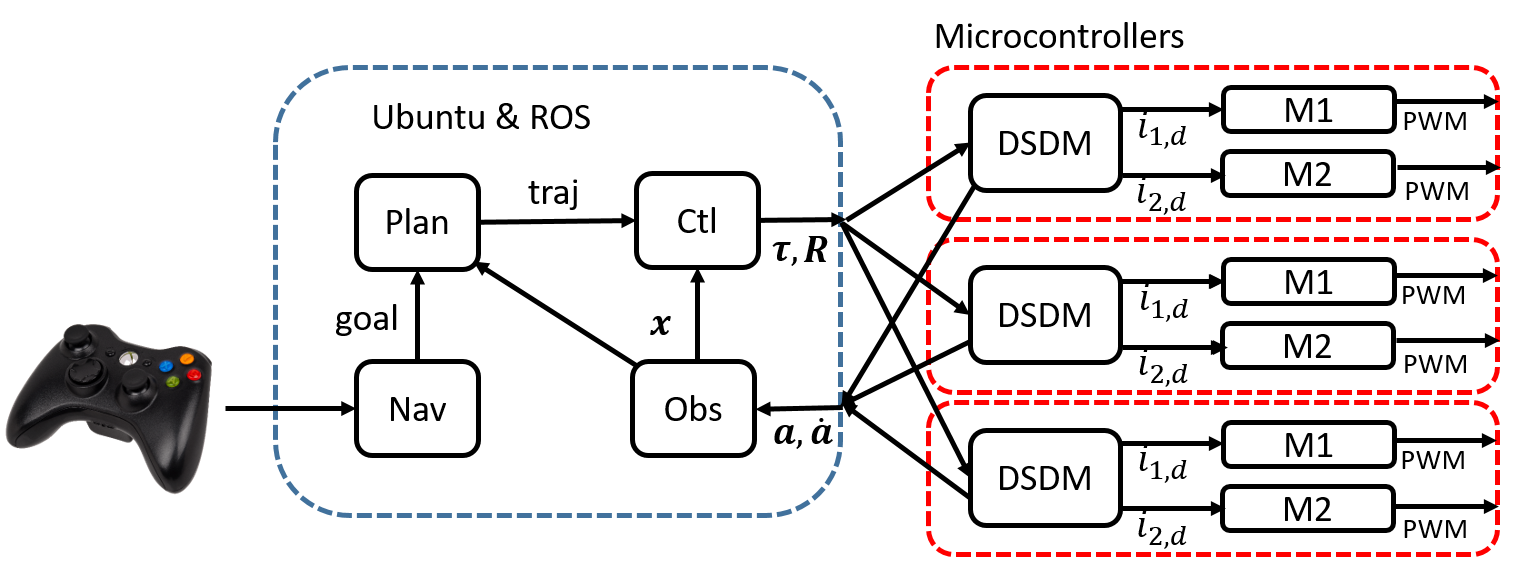
\includegraphics[width=0.95\textwidth]{ros_diagram.png}
	\caption{Control Software Architecture}
	\label{fig:ros_diagram}
\end{figure}


%\subsection{Motor drivers}

\subsection{DSDM Actuator Controllers}

\subsection{Robot Trajectory Following Controller}

\subsection{Motion Planning Algorithm}

